
% this file is called up by thesis.tex
% content in this file will be fed into the main document

% ----------------------- introduction file header -----------------------
\chapter{Data modeling and object reconstruction} 
\label{chapter:object_reco}
Monte Carlo event generators are the indispensable workhorses of particle physics, bridging the gap between theoretical ideas and first-principles calculations on the one hand, and the complex detector signatures on the other hand.
In fact, they are mainly used to predict event rates and topologies, simulate possible backgrounds, study detector requirements and study detector imperfections.\\
The same reconstruction algorithms are used to reconstruct data and all MC samples.

% ----------------------- paths to graphics ------------------------

% the code below specifies where the figures are stored
\graphicspath{Chapters/CH4/figures}

% ----------------------------------------------------------------------
% ----------------------- introduction content -------------------------
% ----------------------------------------------------------------------
\section{Event simulation}
To understand what the final state of any given physics process looks like,
\textit{Monte Carlo simulation} (MC) is used to model both the initial and final state of the 
process of interest, as well as the propagation of particles through the detector. \\
A typical MC simulated $p-p$ collision can be schematized as in Figure~\ref{fig:MC}.
\begin{figure}[h]
	\centering
	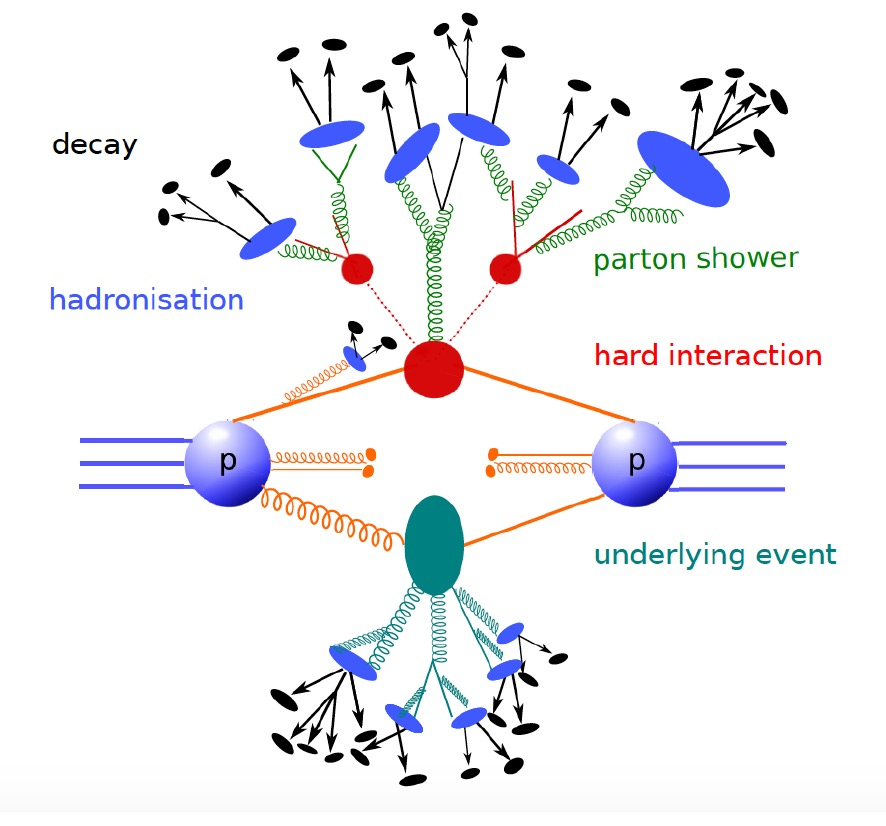
\includegraphics[width=0.7\textwidth]{Chapters/CH4/figures/MC}
	\caption{Typical Monte Carlo simulated event with representation of several processes: underlying event, hard scattering, parton shower, hadronisation and decay.}
	\label{fig:MC}
\end{figure}
\\ The first step of an event simulation is represented by the extraction of initial-state partons and the evaluation of their momenta using the proton PDFs.\\
Fixed order matrix element (ME) are used to determine the cross section for the hard scatter 
integrated over the phase space of the final state particles and it also predicts their momenta.\\
The particles produced by the hard scatter then undergo a process of \textit{parton showering} 
(PS), where the quarks and gluons produce a “shower” of further coloured particles.\\
Particles are emitted and produced until the energy scale is below 1 GeV, at which point, the 
\textit{hadronisation} process starts and colorless hadrons are formed. These hadrons then decay 
into lighter particles.\\
As well as the original hard scatter, additional interactions between other partons within the
proton must be included in a process known as \textit{underlying event}.
\newpage
\noindent Finally, \textit{pile-up} collisions also overlaid, which originate from collisions of other
protons in the beam.
For hadronisation, two main models exist: the string model~\cite{string} and the cluster 
model~\cite{cluster}.\\ In the \texttt{PYTHIA} event generator~\cite{pythia} the string model is used 
whereas the \texttt{HERWIG} event generator~\cite{herwig} uses the cluster model. The 
differences in performance of these models can be used to assess the uncertainty due to the 
model chosen.\\
The output of the MC event generation process is used as an input to a simulation of the
ATLAS detector. This simulation describes all of the detector material and geometry, as
well as any defects in the material or electrical problems. The simulation is built using the
\texttt{GEANT4}~\cite{geant}. simulation software.
The output of the detector simulation is reconstructed in the exact same way as data to allow the 
two to be compared directly.
The simulation of the passage of particles through the detector is very computationally expensive.
This is mainly due to simulation of the calorimeters because it is extremely time consuming
to simulate the particle showers. To speed this up, an approximate simulation, 
\texttt{ATLASFAST-II} (AFII)~\cite{afii}, is often used. This approximate model simulates the 
particle showers in the calorimeters using parameterised functions applied to particle energy, 
rather than carrying out the full shower simulation.

\newpage
\section{Object reconstruction}
This section describes the main reconstruction and identification criteria applied for each physics
objects considered in this analysis (electrons, muons, jets, $b$-tagged jets and missing transverse momentum). \\
A summary of the object selections is reported in~\Cref{tab:objects}.

\begin{table}[!h]
	\scriptsize
	\centering
	\begin{tabular}{cccccl}
		\toprule
		& $p_{T}$ & $|eta|$ & ID & Isolation & Additional cuts \\
		\midrule
		Electrons & $>$ \SI{15}{\GeV} & $<$ 2.47 & \texttt{MediumLH} & \texttt{PLVTight}  & $|d_0^\mathrm{BL}~\mathrm{significance} | < 5$ \\
		& & & & & $|\Delta z_0^\mathrm{BL} \sin\theta| < \SI{0.5}{mm}$ \\
		\midrule
		Muons & $>$ \SI{15}{\GeV} & $<$ 2.5 & \texttt{Medium} & \texttt{PLVTight}  & $|d_0^\mathrm{BL}~\mathrm{significance} | < 5$ \\
		& & & & & $|\Delta z_0^\mathrm{BL} \sin\theta| < \SI{0.5}{mm}$ \\
		\midrule
		Soft Muons & $>$ \SI{4}{\GeV} & $<$ 2.5 & \texttt{Tight} & -- & $|d_0| < \SI{3}{\milli\metre}$ \\
		& & & & & $|z_0 \sin\theta| < \SI{3}{\milli\metre}$ \\
		& & & & & $\Delta R(\mu,\mathrm{jet}) < 0.4$ \\
		\midrule
		Jets & $>$ \SI{25}{\GeV} & $<$ 2.5 & PFlow & --  & JVT \\
		\midrule
		$b$-jets & $>$ \SI{25}{\GeV} & $<$ 2.5 & \texttt{DL1r @\SI{77}{\%}} & --  & --\\
		\bottomrule
	\end{tabular}
	\caption{\normalsize{Overview of the requirements applied for selecting objects.}}
	\label{tab:objects}
\end{table}


% -------------------------------------------------------------------------------
\FloatBarrier
\subsection{Electrons}
\label{sec:object:el}
Electron candidates are reconstructed from energy clusters in the
electromagnetic (EM) calorimeter that match a reconstructed track in
the inner detector (ID)~\cite{ATL-PHYS-PUB-2015-041,ATL-PHYS-PUB-2016-015,ATLAS-CONF-2016-024,PERF-2017-01}.
The clusters are required to be within the range $|\eta| < 2.47$,
excluding the transition region between the barrel and endcap calorimeters at 
$1.37 < |\eta| < 1.52$. 
Electron candidates must also satisfy a
transverse energy requirement of $E_{T} >\SI{15}{\GeV}$. \\
Further requirements on the electromagnetic shower shape, calorimeter
energy to tracker momentum ratio, and other discriminating variables
are combined into a likelihood-based object quality cut (LH), optimised for
strong background rejection. All electron candidates in this analysis
must pass the \texttt{MediumLH} selection.\\
Electron tracks are also required to be consistent with the beam line 
applying the requirements: 
$|d_0^\mathrm{BL}~\mathrm{significance} | < 5$ and 
$|\Delta z_0^\mathrm{BL} \sin\theta| < \SI{0.5}{mm}$. \\
Electrons are further required to be isolated, to reject
candidates coming from other sources than prompt $W$ or
$Z$ boson decays (hadrons faking an electron signature,
heavy-flavour decays or photon conversions). \\
The isolation working point used in this analysis is \texttt{PLVTight}. \\
Correction factors are applied to simulated electrons to take into account the small differences in
reconstruction, identification and isolation efficiencies between data and MC simulation.

% -------------------------------------------------------------------------------
\FloatBarrier
\subsection{Muons}
\label{sec:object:mu}
Muon candidates are reconstructed by combining a reconstructed track
from the ID with one from the muon spectrometer
(MS)~\cite{PERF-2015-10}, and are required to have $p_{T}>\SI{15}{\GeV}$
and $|\eta|<2.5$. \\
The different combinations of input information (from ID and MS) leads to four different
types of reconstructed muons:
\begin{itemize}
\item \textbf{Combined muons (CB)}: a combined track is formed reconstructing independently tracks in the ID and MS;
\item \textbf{Segment-tagged muons (ST)}: a track in the ID is classified as a muon if, once
extrapolated to the MS, it is associated with at least one local track segment
in the MDT or CSC chambers;
\item \textbf{Calorimeter-tagged muons (CT)}: classification for ID tracks that are matched to an 
energy deposit in the calorimeter and it is compatible to a minimum ionising particle;
\item \textbf{Extrapolated muons (ME)}: the reconstructed trajectory of ME muons uses only the
MS track and some loose requirement that its origin is the interaction point;
\end{itemize}
Muons from $Z$ or $W$ boson decays are considered $prompt$ muons whereas those
coming from pion or kaon decays are $non-prompt$ muons. \\
This analysis needs the suppression of the contribution from non-prompt muons, therefore 
requirements are placed on muon candidates. \\
In CB tracks, the variables commonly used in muon identification are:
\begin{itemize}
	\item $\bm{q/p}$ \textbf{significance}: defined as the absolute value of the difference between the
ratio of the charge and momentum of the muons measured in the ID and MS
divided by the sum in quadrature of the corresponding uncertainties;
	\item $\bm{\rho'}$: defined as the absolute value of the difference between the transverse momentum
measurements in the ID and the MS divided by the $p_T$ of the combined
track;
	\item $\bm{\chi^2}$: normalised $\chi^2$ of the combined track fit.
\end{itemize}
To reject misidentified muon candidates, primarily originating from pion and kaon decays, several 
quality requirements can be imposed on the muon candidate.\\
There are four muon identification working points:
\begin{itemize}
	\item \textbf{Tight Muons}: selected to maximise the purity of muons
at the cost of some efficiency. Only CB muons with hits in at least two stations
of the MS and satisfying the Medium selection criteria are considered.
The reconstruction efficiency for Tight muons in the range $20 < p_T < 100$ GeV is 91.8\%.
	\item \textbf{Medium Muons}: this is the default working point used by the ATLAS collaboration.
Only CB and ME tracks are used. The CB tracks are required to have 3 hits in at
least two MDT layers. The reconstruction efficiency for this working point in
the range $20 < p_T < 100$ GeV is 96.1\%.
	\item \textbf{Loose Muons}: all CB and ME muons that satisfy the Medium requirement are also
included in the Loose selection. It is optimised to maximise the reconstruction efficiency, while 
still retaining only good quality muon tracks. The reconstruction efficiency for
Loose muons in the range $20 < p_T < 100$ GeV is 98.1\%.
	\item \textbf{High-$\bm{p_T}$ Muons}: the selection is optimised for analyses searching for
high-mass resonances using muons. CB muons are required to pass the Medium selection
and have at least three hits in three MS stations. This selection maximises the momentum
resolution for muons with pT > 100 GeV
\end{itemize}
The muon candidates in this analysis must pass the \texttt{Medium}
identification definition, already described above.\\
Muon tracks are also required to be consistent with the beam line
applying the requirements: 
$|d_0^\mathrm{BL}~\mathrm{significance} | < 3$ and 
$|\Delta z_0^\mathrm{BL} \sin\theta| < \SI{0.5}{mm}$. \\
Muons are further required to be isolated and the isolation working point used in this analysis is \texttt{PLVTight}.\\
Like for electrons, correction factors are applied to simulated muons
to account for the small differences between data and simulation. 

\subsection{Soft muons}
\label{sec:object:soft_muons}
Different requirements are applied to select and distinguish muons 
from leptonic decays of the Z and W bosons 
(referred to as`prompt' or `isolated' muons in the following) 
and muons from semi-leptonic c-hadron decays 
(called `soft' or `SMT' muons in the following). \\
Reconstructed muons with $p_{T} > 4 $ GeV not passing 
the prompt muon selection can instead be selected as soft muons.\\
Soft muons are required to pass the \texttt{Tight} quality requirements~\cite{muon2015} 
and to be closer than 0.25 in $\Delta R$ within a selected jet. 
%In case more than one muon passing these criteria is found for a given jet,
%the soft muon with the lower $p_{T}$ is chosen. 
The closest jet to a soft muon is defined as the `SMT' jet. \\
Very loose requirements are applied on the impact parameters to remove
pathological cases: 
$|d_0| < 3$ mm and $|z_0 \sin\theta| < 3$  mm.
More details on the soft muon tagging are in Ref.~\cite{SMT-INT-13TeV}.

\FloatBarrier
\subsection{Jets}
\label{sec:object:jet}
Jets are reconstructed 
using the particle flow algorithm~\cite{PERF-2015-09}. \\
All jets considered in this analysis should have a transverse
momentum $p_{T} > 25$ GeV and a pseudo-rapidity of
$|\eta|\!<\!2.5$.\\
To suppress jets from in-time pileup, the \texttt{Jet Vertex Tagger} (JVT)
discriminant, which is based on a two-dimensional likelihood
method, is used~\cite{ATLAS-CONF-2014-018}. A JVT value of at least
0.59 is required for jets with $p_{T}< 60$ GeV
and $|\eta|\!<\!2.4$, corresponding to an efficiency of 92\%.

%\subsection{Jet Flavour Tagging }

\subsection{Soft Muon Tagging}
\label{sec:object:smt}
The Soft Muon Tagging (SMT) is a tagging technique for heavy-flavour jets.\\
 It exploits the $b \rightarrow \mu + X$,
 $b \rightarrow c \rightarrow \mu + X$ and $c \rightarrow \mu + X$ decay chains (with a total BR$\approx$ 20\%), by identifying muons reconstructed inside jets. Those muons are referred to as soft muons and they were described in Section~\ref{sec:object:soft_muons}.
 More details on the soft muon tagging are in Ref.~\cite{SMT-INT-13TeV}.

\subsection{Recurrent Deep-Learning DL1r}
In this analysis the \texttt{DL1r} algorithm is used~\cite{ATL-PHYS-PUB-2017-013,Aad:2019aic}.
It is based on a deep feed-forward neural network (NN) trained using Keras~\cite{keras} with the Theano~\cite{theano} backend and the Adam optimiser~\cite{adam}. The DL1 NN has a multidimensional output corresponding to the probabilities for a jet to be a b-jet, a c-jet or a light-flavour jet. The topology of the output consists of a mixture of fully connected hidden and Maxout layers~\cite{goodfellow2013maxout}. The input variables to DL1 consist of those used for the previous official algorithm MV2, with the addition of the \textsc{JetFitter} c-tagging variables described in Ref.~\cite{Aad:2019aic}.
\subsubsection {\textit{b}-tagged jets}
\label{sec:object:bjet}
Jets originating from bottom quarks (called $b$-tagged jets) are
identified by reconstructing secondary vertices from the tracks
associated to the jets and by combining their spatial parameters with
life-time related information.
In the current  analysis the \SI{77}{\%} operation point is used.\\
Finally, all $b$-tagged jets considered in this analysis should have a transverse
momentum $\pT > \SI{25}{\GeV}$ and a pseudo-rapidity of
$|\eta|\!<\!2.5$.  
\subsubsection {\textit{c}-tagged jets}
\label{sec:object:cjet}
The \texttt{DL1r} algorithm also allows to construct DL1r$_{c}$ discriminant that is used for charm-tagging.\\
They are reconstructed jets satisfying $\pT > \SI{25}{\GeV}$ and $|\eta| < 2.5$ requirements,
and failing the $b$-tagging requirement.
This search uses the cut operation point giving the $c$-efficiency of 20\% studied and being calibrated
in the $tc$+MET SUSY analysis~\cite{ANA-SUSY-2019-23}.\\
More details of charm-tagging are given in~\Cref{appendix:DL1rc}.

\subsection{Missing transverse momentum}
\label{sec:object:met}
The missing transverse momentum, $E^{miss}_{T}$, is a measure of the momentum
imbalance, usually due to escaping neutrinos. 
It is calculated as the magnitude of the negative vector sum of the momenta 
in the transverse plane of all selected calibrated physics objects in the event~\cite{MTM1,MTM2}. \\
To account for the soft hadronic activity, a soft term built from
tracks that are associated to the hard-scatter vertex but are not
associated to any of the reconstructed objects. The soft term is
included in order to account for low-momentum particles that are not
identified among the final state objects~\cite{PERF-2011-07,PERF-2014-04,ATL-PHYS-PUB-2015-027}.\\
It also includes an extra term to account energy losses due to the detector inefficiencies 
and resolution leading to the mis-measurement of the true transverse energy of the final 
interacting objects.

\subsection{Overlap removal}
\label{sec:object:over_rem}
In order to avoid double counting of single final state objects, like e.g. an 
isolated electron being reconstructed both as an electron and as a jet with the 
requirements above, a procedure is followed to remove overlaps between final state objects. 
This is the sequence of operation that are performed to solve these ambiguities, as 
implemented as the harmonized option~\cite{Adams:1743654} in the \texttt{AssociationUtils}~\cite{AssociationUtils} package:
\begin{itemize}
	\item Electron candidates which share a track with a muon candidate are remove.
	\item If the distance in $\Delta R$ between a jet and an electron candidate 
	is $\Delta R < 0.2$, then the jet is dropped. If multiple jets are found with this requirement, 
	only the closest one is dropped.
	\item If the distance in $\Delta R$ between a jet and a baseline
	electron is $0.4 < \Delta R < 0.2$, 
	then the electron is dropped.
	\item If the distance in $\Delta R$ between a jet and a muon
	candidate is $\Delta R < 0.4$, then: if 
	the jet has more than 2 associated tracks then the muon is dropped, otherwise the jet is removed.
\end{itemize}
No overlap removal is performed on muons used for the Soft Muon Tagging.


\label{soft_mu}


\clearpage
